\documentclass[tikz,border=6pt]{standalone}
\usepackage[T1]{fontenc}
\usepackage{lmodern}
\usetikzlibrary{arrows.meta,positioning,calc}

\definecolor{modelblue}{HTML}{4C78A8}
\definecolor{transferpurple}{HTML}{8B6BB1}
\definecolor{physicalgreen}{HTML}{59A14F}
\definecolor{ink}{HTML}{303840}

\begin{document}
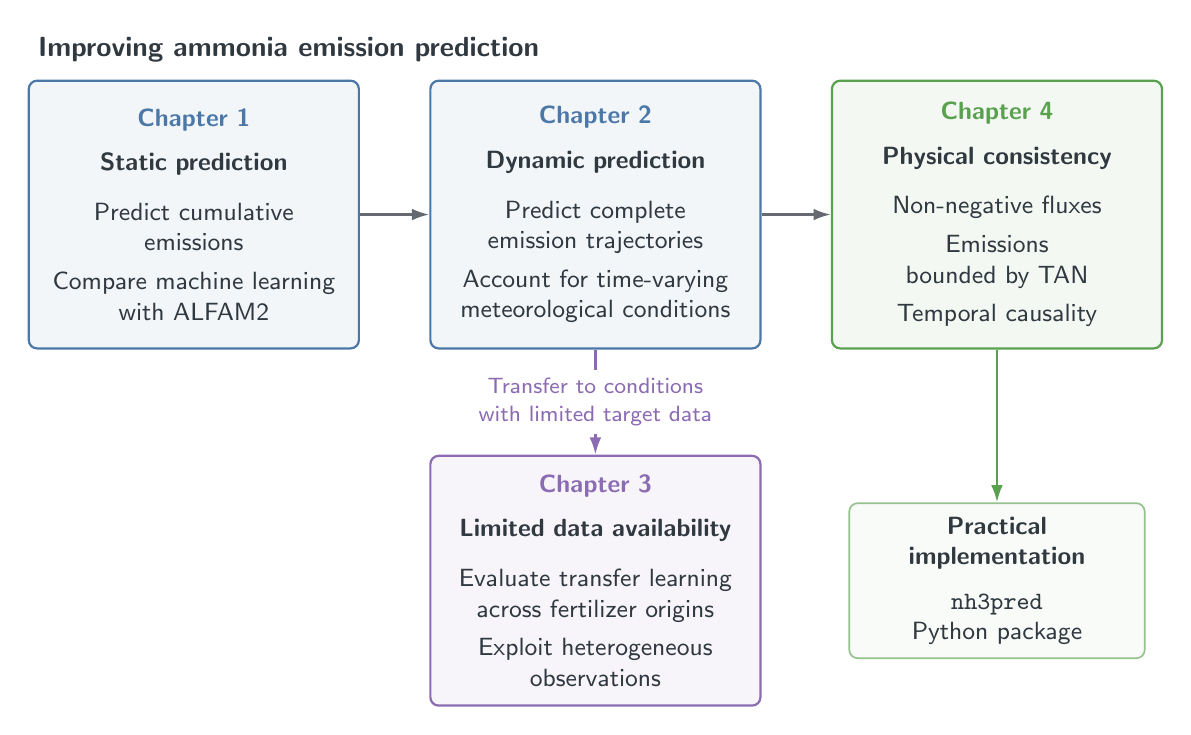
\begin{tikzpicture}[
  font=\sffamily\fontsize{9}{11}\selectfont,
  text=ink,
  card/.style={draw=#1, fill=#1!7, line width=0.8pt,
    rounded corners=3pt, text width=37mm, minimum height=34mm,
    inner sep=7pt, align=center},
  flow/.style={-{Latex[length=2.2mm,width=1.5mm]},
    draw=ink!75, line width=0.9pt},
  label/.style={font=\sffamily\fontsize{8}{10}\selectfont,
    align=center, fill=white, inner sep=3pt}
]

% Main progression: fixed coordinates keep the three chapters aligned.
\node[anchor=west, font=\sffamily\bfseries\fontsize{10}{12}\selectfont]
  at (-2.1,2.1) {Improving ammonia emission prediction};

\node[card=modelblue] (ch1) at (0,0) {
  {\color{modelblue}\bfseries Chapter 1}\\[5pt]
  {\bfseries Static prediction}\\[7pt]
  Predict cumulative\\emissions\\[3pt]
  Compare machine learning\\with ALFAM2
};
\node[card=modelblue] (ch2) at (5.1,0) {
  {\color{modelblue}\bfseries Chapter 2}\\[5pt]
  {\bfseries Dynamic prediction}\\[7pt]
  Predict complete\\emission trajectories\\[3pt]
  Account for time-varying\\meteorological conditions
};
\node[card=physicalgreen] (ch4) at (10.2,0) {
  {\color{physicalgreen}\bfseries Chapter 4}\\[5pt]
  {\bfseries Physical consistency}\\[7pt]
  Non-negative fluxes\\[3pt]
  Emissions bounded by TAN\\[3pt]
  Temporal causality
};
\draw[flow] (ch1.east) -- (ch2.west);
\draw[flow] (ch2.east) -- (ch4.west);

% Complementary research direction, based on the dynamic framework.
\node[card=transferpurple, minimum height=28mm] (ch3) at (5.1,-4.65) {
  {\color{transferpurple}\bfseries Chapter 3}\\[5pt]
  {\bfseries Limited data availability}\\[7pt]
  Evaluate transfer learning\\across fertilizer origins\\[3pt]
  Exploit heterogeneous\\observations
};
\draw[flow, draw=transferpurple] (ch2.south) --
  node[label, text=transferpurple] {Transfer to conditions\\with limited target data}
  (ch3.north);

% Software is an outcome, visually subordinate to the research chapters.
\node[draw=physicalgreen!65, fill=physicalgreen!4,
  rounded corners=3pt, line width=0.6pt,
  text width=34mm, minimum height=16mm, inner sep=5pt, align=center]
  (package) at (10.2,-4.65) {
    {\bfseries Practical\\implementation}\\[5pt]
    \texttt{nh3pred}\\Python package
  };
\draw[flow, draw=physicalgreen] (ch4.south) -- (package.north);

\end{tikzpicture}
\end{document}
